\documentclass[14pt,fleqn]{extarticle}
\usepackage[T2A,T1]{fontenc}
\usepackage[utf8]{inputenc}
\usepackage[russian]{babel}
\usepackage{amsmath}
\usepackage{graphicx}
\usepackage{tabularx}
\usepackage{boldline}
\usepackage{makecell}
\usepackage{arydshln}
\usepackage{mathtools}
\usepackage{centernot}
\usepackage{enumitem}
\usepackage{nccmath}
\usepackage{amssymb}
\usepackage[a4paper, total={6.5in, 9.5in}]{geometry}

\graphicspath{ {./images/} }
\setlength{\mathindent}{0pt}
\setlength\parindent{0pt}

\def\at{
	\left.
	\vphantom{\int}
	\right|
}


\begin{document}
	\begin{titlepage}
		
\includegraphics[scale=0.12]{logo}
		\begin{center}
			\textbf{МИНОБРНАУКИ РОССИИ}\\
			\vspace{0.2cm}
			\textbf{Федеральное государственное бюджетное образовательное учреждение высшего образования}\\
			\textbf{<<САНКТ-ПЕТЕРБУРГСКИЙ ГОСУДАРСТВЕННЫЙ ЭКОНОМИЧЕСКИЙ УНИВЕРСИТЕТ>>}\\
			\vspace{0.6cm}
			Факультет информатики и прикладной математики\\
			Кафедра прикладной математики и экономико-математических методов\\
			\vspace{1cm}
			\textbf{ОТЧЁТ}\\
			по дисциплине:\\
			\textbf{<<Модели экономической динамики>>}\\
			на тему:\\
			\textbf{<<Количественный анализ модели Солоу с человеческим капиталом. Задание №2>>}\\
		\end{center}
		\vspace{1cm}
		Направление: 01.03.02\\
		Обучающийся: Бронников Егор Игоревич\\
		Группа: ПМ-1901\\
		\vfill
		\begin{center}
			Санкт-Петербург\\
			2022\\
		\end{center}
	\end{titlepage}
    \subsection*{Задание}
    Провести количественный анализ модели Солоу с человеческим капиталом.\\
    \newline

    \textit{Модель Солоу с человеческим капиталом в относительных показателях:}\\
    
    $Y$ -- валовый внутренний продукт (ВВП)\\
    $K$ -- физический капитал\\
    $H$ -- человеческий капитал\\
    $L$ -- трудовые ресурсы\\
    $A$ -- технологический прогресс\\
    $s_K$ -- доля инвестиций на физический капитал\\
    $s_H$ -- доля инвестиций на человеческий капитал\\
    $\delta$ -- доля износа\\
    $n$ -- постоянный прирост трудовых ресурсов\\
    $g$ -- постоянный прирост технологического прогресса\\
    $\alpha$ -- эластичность выпуска по физическому капиталу\\
    $\beta$ -- эластичность выпуска по человеческому капиталу\\
    
	\begin{align*}
		& y = k^\alpha \cdot h^\beta\\
		& \dfrac{dk}{dt} = s_K \cdot y - (n + g + \delta) k\\
		& \dfrac{dh}{dt} = s_H \cdot y - (n + g + \delta) h\\
	\end{align*}

	\newpage
	В соответствии с формулами, данная модель была реализована в среде моделирования AnyLogic. В качестве начальных параметров было принято решение взять $\alpha = 0.5$, $\beta = 0.2$, $s_K = 0.6$, $s_H = 0.9$, $\delta = 0.01$, $n = 0.3$, $g = 0.2$, $k_0 = 7$, $h_0 = 14$. (Рисунок \ref{fig:M-R-W_anylogic})
	\begin{figure}[h]
		\centering 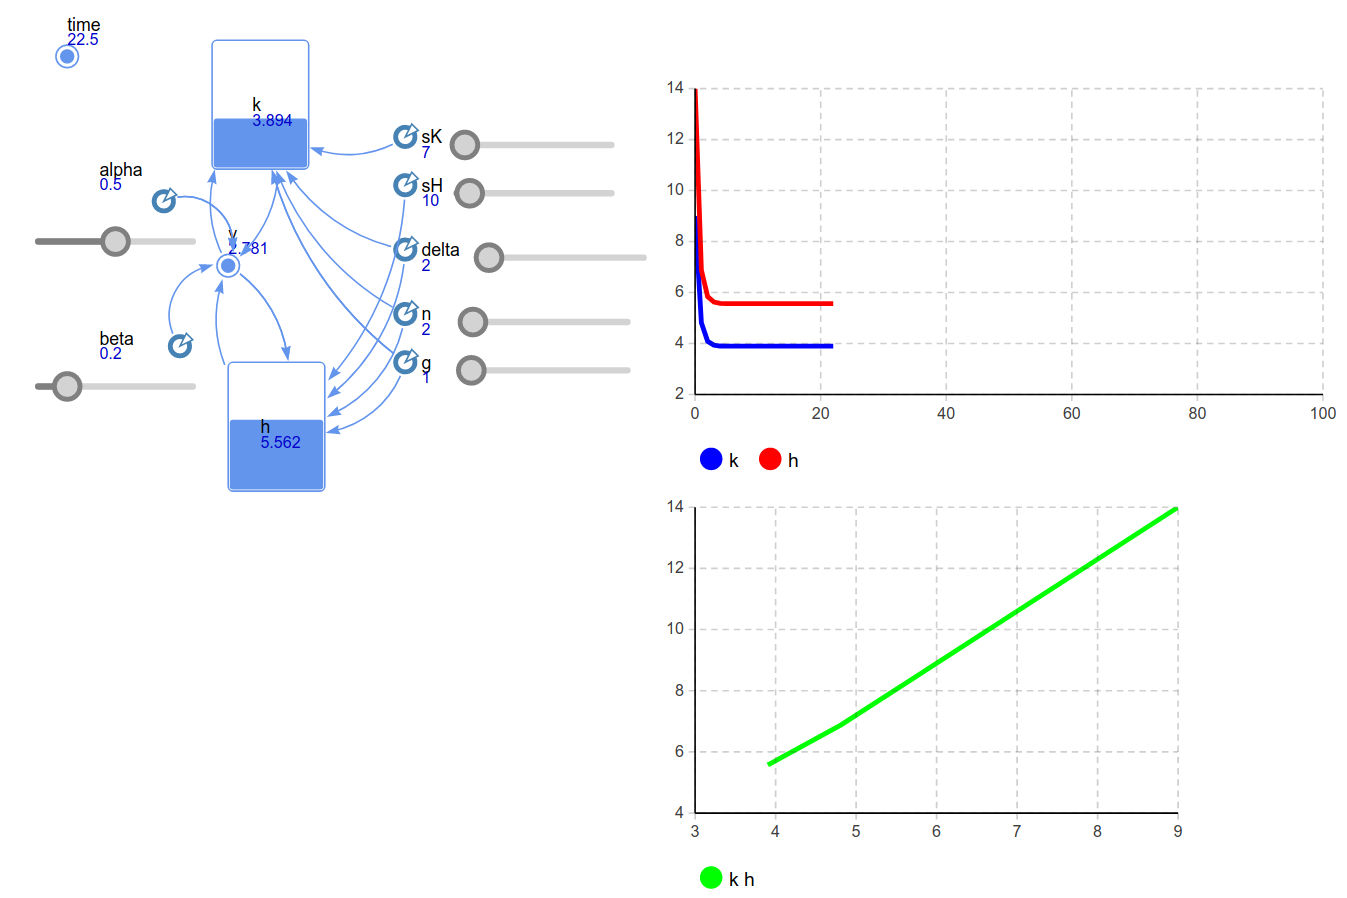
\includegraphics[scale=0.3]{M-R-W_anylogic}
		\caption{Результаты построения модели Солоу с человеческим капиталом в AnyLogic}
		\label{fig:M-R-W_anylogic}
	\end{figure}
	
	Как можно заметить на графике, который демонстрирует изменение физического капитала и изменение человеческого капитала с течением времени, изначально имел место спад, а затем система пришла в стационарное состояние.
	
	\newpage
	Также данная модель была реализована на языке программирования Python. Для решения системы дифференциальных уравнений был реализован и применён метод Рунге-Кутта. (Рисунок \ref{fig:M-R-W_runge_kutta})
	\begin{figure}[h]
		\centering 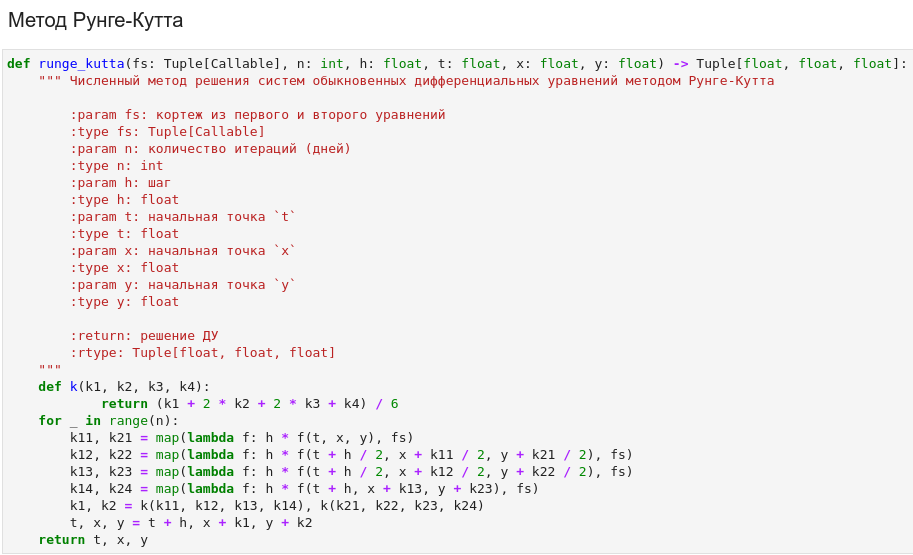
\includegraphics[scale=0.5]{M-R-W_runge_kutta}
		\caption{Метод Рунге-Кутта на языке программирования Python}
		\label{fig:M-R-W_runge_kutta}
	\end{figure}
	
	Параметры модели были взяты из AnyLogic. (Рисунок \ref{fig:M-R-W_python_result})
	\begin{figure}[h]
		\centering 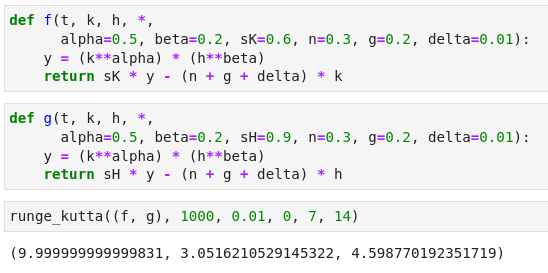
\includegraphics[scale=0.5]{M-R-W_python_result}
		\caption{Результаты построения модели Солоу с человеческим капиталом в Python для десятого момента времени}
		\label{fig:M-R-W_python_result}
	\end{figure}
	
	\newpage
	
	На основании полученных результатов можно построить график, который демонстрирует изменение физического капитала ($k$) и изменение человеческого капитала ($h$) с течением времени. (Рисунок \ref{fig:M-R-W_python_result_plot})
	\begin{figure}[h]
		\centering 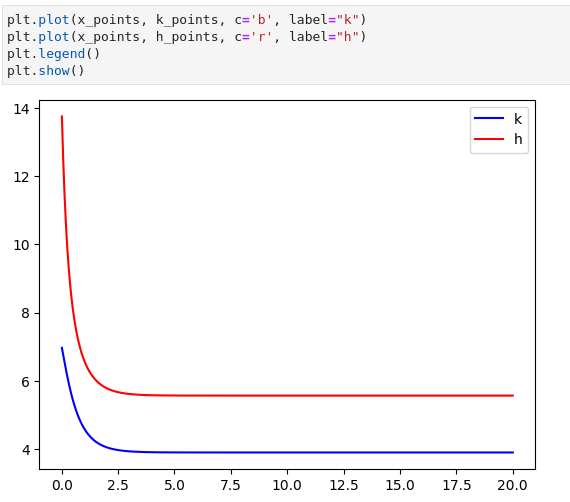
\includegraphics[scale=0.4]{M-R-W_python_result_plot}
		\caption{График изменение капиталов модели}
		\label{fig:M-R-W_python_result_plot}
	\end{figure}
	
	Как можно заметить данный график полностью соответствует графику, который был построен с помощью инструмента AnyLogic.\\
	
	Также если изменять параметры модели, то она всё равно будет приходить в устойчивое состояние. (Рисунок \ref{fig:M-R-W_anylogic_variance})
	\begin{figure}[h]
		\centering 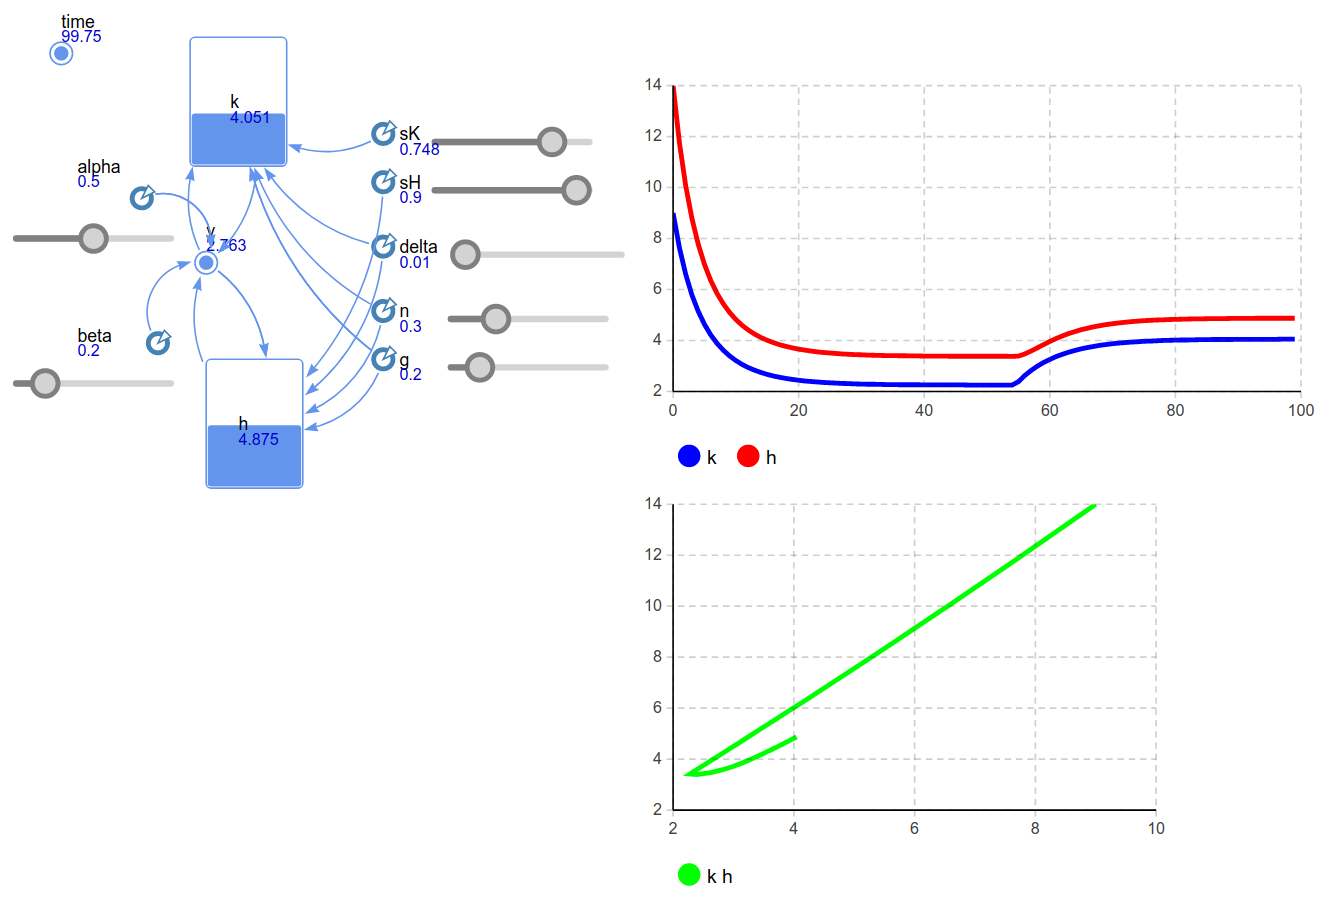
\includegraphics[scale=0.25]{M-R-W_anylogic_variance}
		\caption{Изменение параметров модели}
		\label{fig:M-R-W_anylogic_variance}
	\end{figure}
\end{document}
